\documentclass{article}

\usepackage[english,french]{babel}
\usepackage[utf8]{inputenc}
\usepackage[T1]{fontenc}
\usepackage{amsmath, amsfonts, amssymb, amsthm}
\usepackage{bbm,algorithmic,algorithm,verbatim}
\usepackage{color}
\usepackage{subcaption}
\usepackage[pdftex]{graphicx}
\usepackage{epsfig}
\usepackage{ulem, stmaryrd, dsfont}
\usepackage{scribe}
\usepackage{shortcuts_js}

\PassOptionsToPackage{hyphens}{url}
\usepackage[pdftex,linkcolor=test,citecolor=vsomb_col,
colorlinks=true,pagebackref,bookmarks=true,plainpages=true,
urlcolor=fb_col]{hyperref}
\usepackage{cleveref}

\begin{document}
\sloppy
\lecture{HMMA307}{
Linear mixed effects models}{Catherine Baltazar, Dalal Hanna, Jacob Ziegler}{Cassandre Lepercque}


%%%%%%%%%%%%%%%%%%%%%%%%%%%%%%%%%%%%%%%%%%%%%%%%%%%%%%%%%%%%%%%%%%%%%%%%%%%%%%%
%%%%%%%%%%%%%%%%%%%%%%%%%%%%%%%%%%%%%%%%%%%%%%%%%%%%%%%%%%%%%%%%%%%%%%%%%%%%%%%
\section{Introduction}
\label{sec:introduction}

A mixed model or mixed-effects model is a statistical model containing both fixed effects and random effects.These models are useful in a wide variety of disciplines in the physical, biological and social sciences. \\
Mixed effects models allow ecologists to overcome a number of limitations associated with traditional linear models.\\
In our case, we will use this model on an environmental data set. In this project, we will do a linear mixed model analysis, check its assumptions, report results, and visually represent our model.\\

Biological and ecological data are often messy. Usually, there is a particular structure to data and we know that relationships between variables of interest might differ depending on grouping factors like species, and more often than not sample sizes are low making it difficult to fit models that require many parameters to be estimated. Linear mixed model (lmm) are made to deal with these problems.

\subsection{Objectives}
\begin{enumerate}
    \item What is a linear mixed effects model (LMM) and why should I care?
    \item How do I implement LMM's in Python ?
    \begin{enumerate}
        \item A priori model building and data exploration
        \item Potential models and model selection
        \item Model validation
        \item Interpreting results and visualizing the model
    \end{enumerate}
\end{enumerate}

\section{What is a linear mixed effects model and why should I care?}
LMM's allow you to use all the data you have instead of using means of non-independent samples, they account for structure in your data, they allow relationships to vary by different grouping factors, and they require less parameter estimates than classical regression.

\subsection{Introduction to the dataset}
The dataset we will be using deals with fish trophic positions. The trophic position of an organism is the place it occupies within the food chain. Three species were selected for the study and ten individuals per species were measured (body length) in six different lakes. Here is a visual representation of the dataset. \\
Note: only three individuals are shown per species, but in reality there are 10 individuals per species.
\begin{figure}[h!]
    \centering
    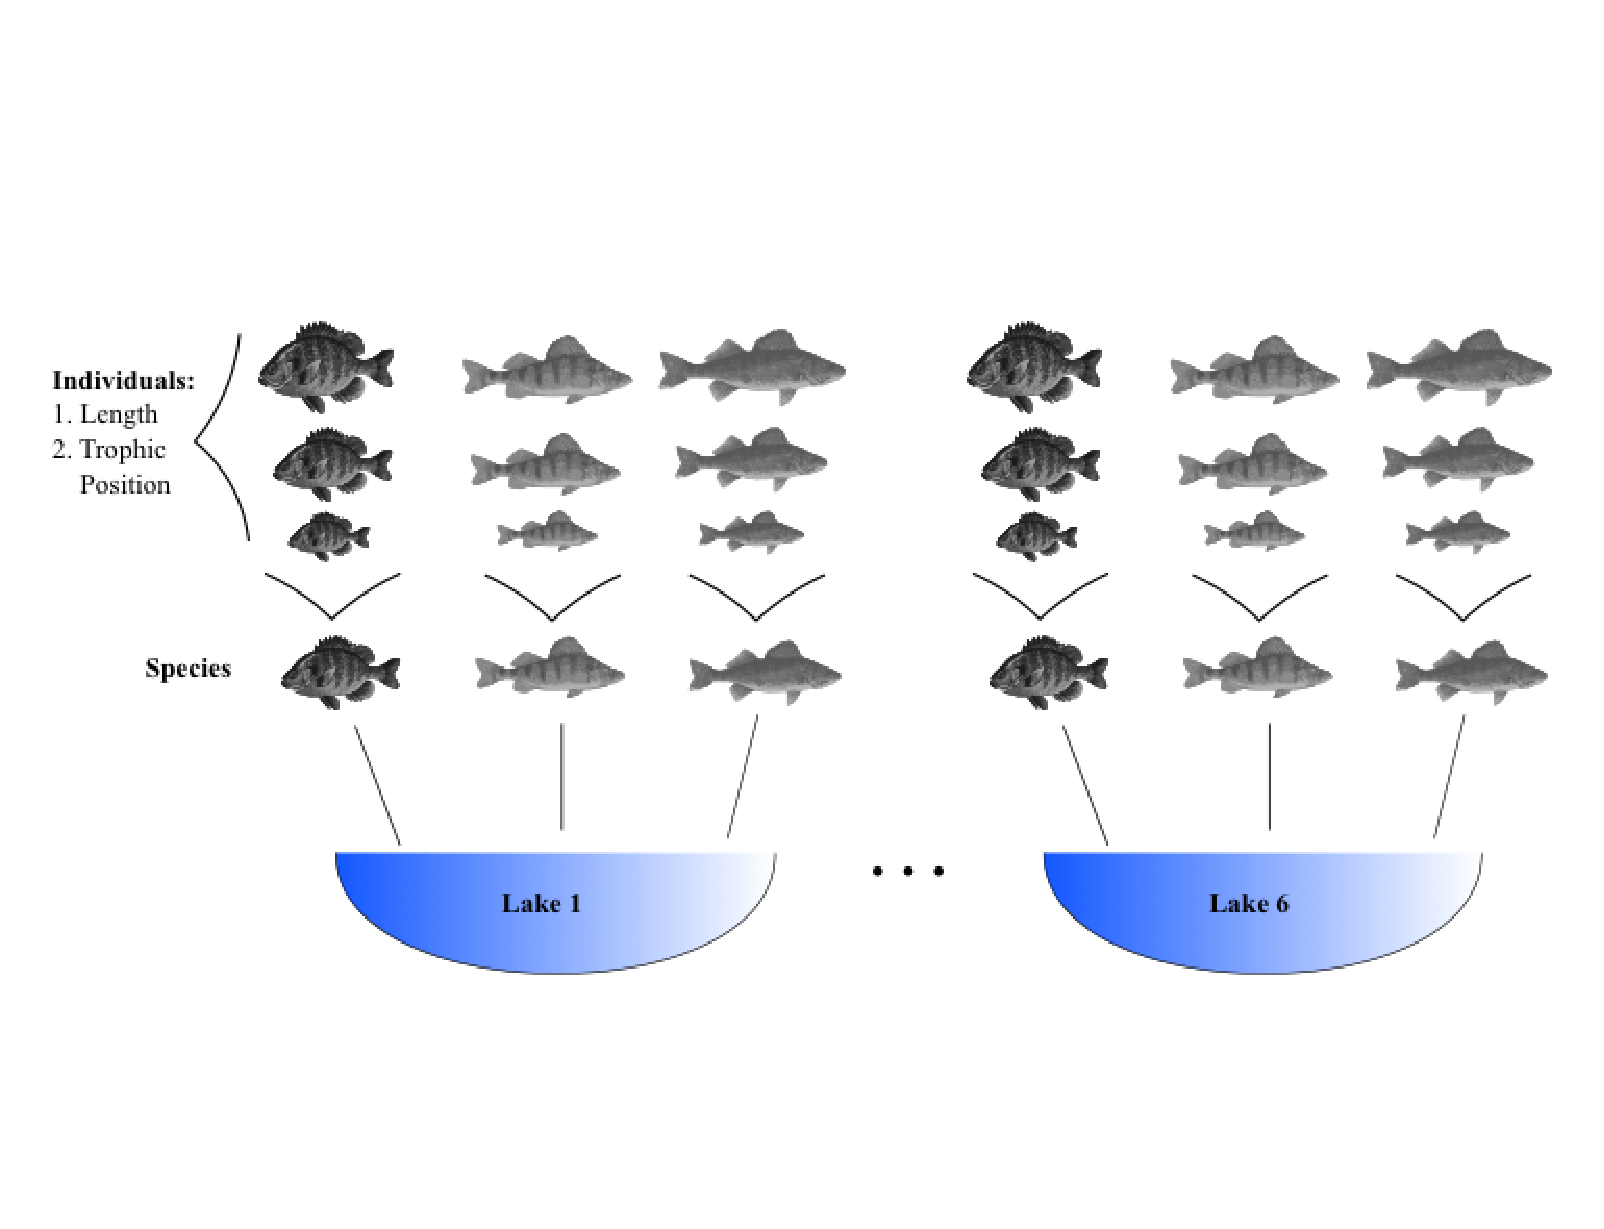
\includegraphics[scale = 0.5]{images/fish_repartition.pdf}
    \caption{Fish dataset.}
    \label{Fish_dataset}
\end{figure}

\subsection{Random and Fixed effects}
There are many possible definitions, and we chose to present those we think are easier to apply.
\subsubsection{Fixed effects}
When a variable has a fixed effect, data is usually gathered from all it's possible levels. The person doing the analyses is also interested in making conclusions about the levels for which the data was gathered.
\subsubsection{Random effects}
Variables with a random effect are also called random factors, as they are only categorical variables (not continuous variables). A random effect is observed when the data only includes a random sample of the factor's many possible levels, which are all of interest. They usually are grouping factors for which you want to control the effect in your model, but are not interested in their specific effect on the response variable.

\subsection{How LMM's works ?}
By definition, in matrix notation, a linear mixed model can be represented as, 
\begin{equation*}
    y = X \beta + Z u + \epsilon
\end{equation*}
where,
\begin{itemize}
    \item $y$ is  a known vector of observations, with mean $\bbE[y]=X \beta$,
    \item $\beta$ is an unknown vector of fixed effects,
    \item $u$ is an unknown vector of random effects, with mean $\bbE[u] = 0$,
    \item $\epsilon$ is an unknown vector of random errors, with mean $\bbE[\epsilon]=0$,
    \item $X$ and $Z$ are known design matrices relating the observations $y$ to $\beta$ and $u$,  respectively.
\end{itemize}

\subsubsection{ Intercepts and/or slopes are allowed to vary by lake and species}
In LMM's allowing intercepts and/or slopes to vary by certain factors (random effects) simply means you assume they come from a normal distribution. A mean and standard deviation of that distribution are estimated based on your data. The most likely intercepts and slopes from that distribution are then fit by optimization (ex. maximum likelihood or restricted maximum likelihood).

\subsubsection{ Intercepts, slopes, and associated confidence intervals are adjusted to account for the structure of data}
If a certain species or a lake is poorly represented (small sample) in the data, the model will give more importance to the grouped model to estimate the intercept and the slope of this species or this lake.\\
Confidence intervals of intercepts and slopes are adjusted to account for pseudoreplication based on the intraclass correlation coefficient (ICC). An adjusted sample sized based on how correlated the data within groups are.\\
Let's see how it goes when we have high ICC or low ICC.
\begin{figure}[h!]
    \begin{minipage}[c]{0,3\textwidth}
    \centering
    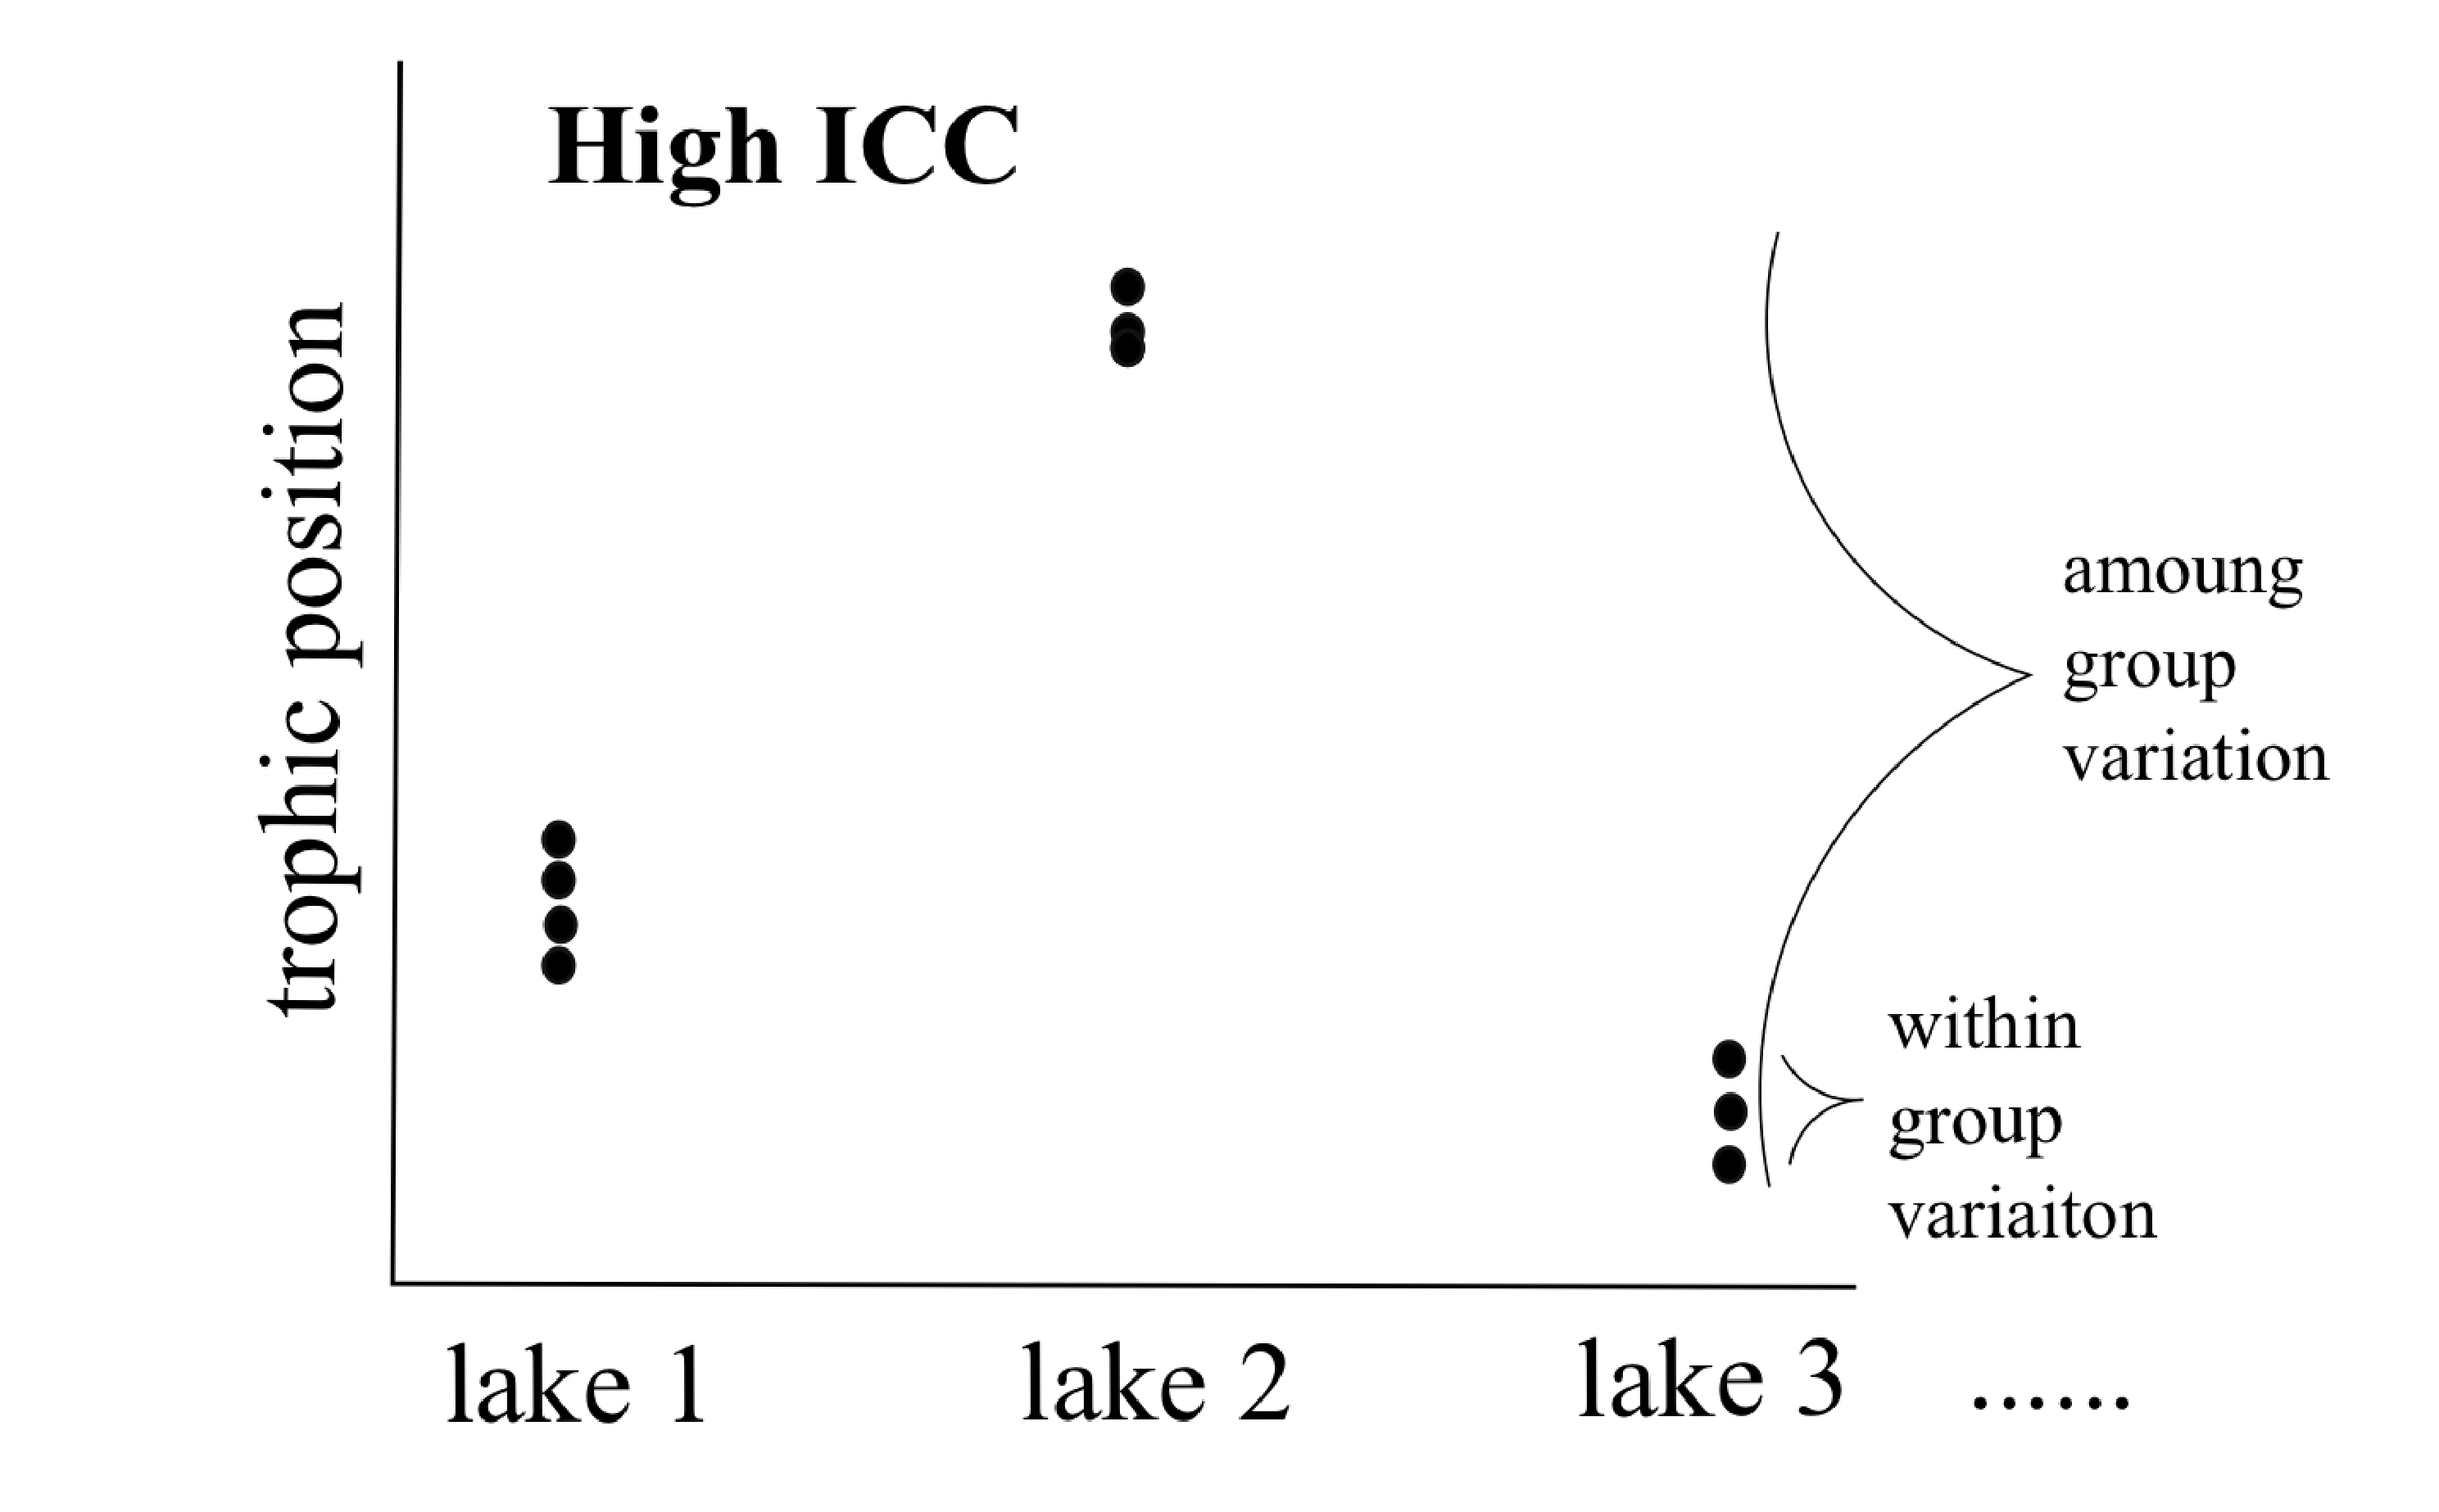
\includegraphics[scale = 0.15]{images/high_CIC.pdf}
    \caption{High ICC representation}
    \label{High_icc}
    \end{minipage}
    \begin{minipage}[c]{0,9\textwidth}
    \centering
    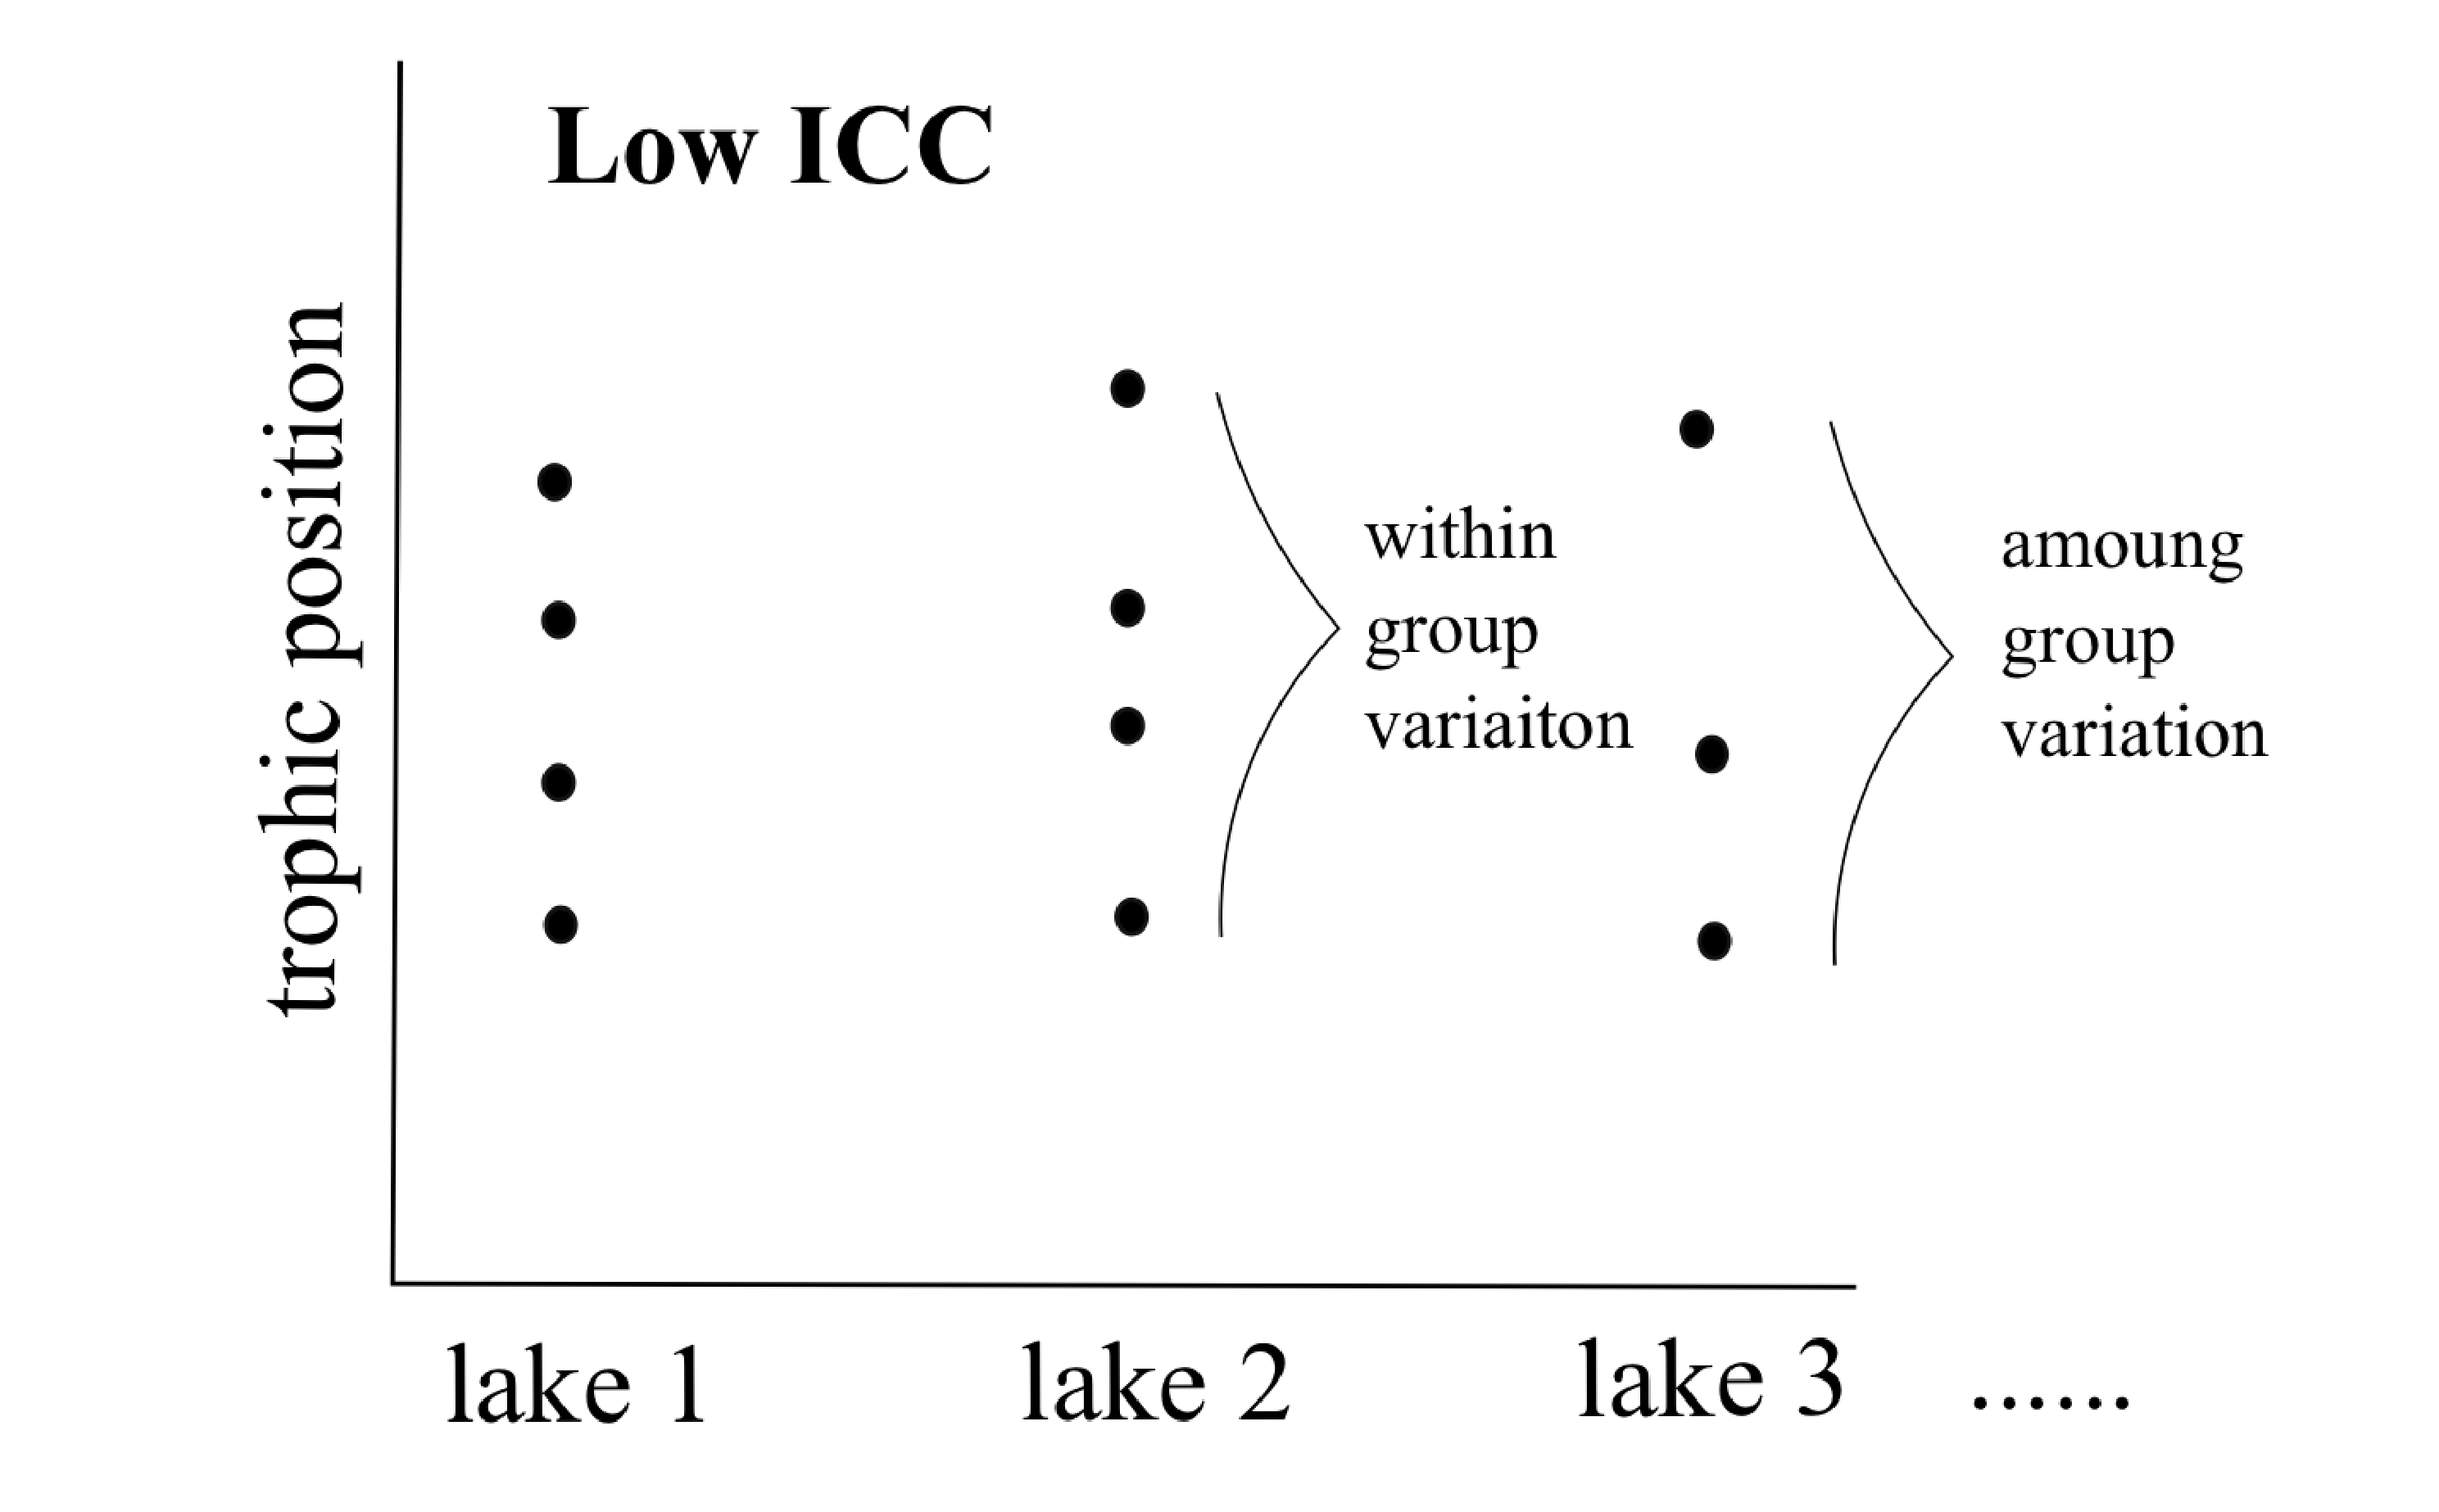
\includegraphics[scale = 0.15]{images/low_CIC.pdf}
    \caption{Low ICC representation}
    \label{Low_icc}
    \end{minipage}
\end{figure}

In Figure \ref{High_icc}, the LMM will treat points within lake more like an overall mean because they are highly correlated. Therefore, the effective sample size will be smaller leading to larger confidence intervals around your slope and intercept parameters.\\
In Figure \ref{Low_icc},  the LMM will treat points within lake more independently because things are less correlated within groups compared to among groups. Therefore the effective sample size will be larger leading to smaller confidence intervals around your slope and intercept parameters.

\section{How do I implement LMM’s in Python ?}
We now going to see how to implement LMM's in Python.

\subsection{A priori model building and data exploration}
We want to determine if trophic position can be predicted by body length, while taking into account variation between species and lakes. So, we have the following model,
\begin{equation*}
    TP_{ijk} \sim Length_i + Lake_j + Species_k + \epsilon ,
\end{equation*}
where,
\begin{itemize}
    \item $TP_{ijk}$ is the trophic position of individual $i$ from lake $j$ of species $k$,
    \item $\epsilon$ are the residuals of the model.
\end{itemize}

We first look at the distribution of samples for each factor, and it's going like this :

\begin{table}[h!]
   \centering
    \begin{tabular}{ |p{2cm}||p{2cm}|p{2cm}|p{2cm}|p{2cm}|p{2cm}|p{2cm}|}
    \hline
    \textbf{Lake} & L1 & L2 & L3 & L4 & L5 & L6 \\
    \hline
     & 30 & 30 & 30 & 30 & 30 & 30\\ 
    \hline
    \hline
    \textbf{Species} & S1 & S2 & S3 & & & \\
    \cline{1-4}
     & 60 & 60 & 60 & & & \\
     \hline
    \end{tabular}
    \caption{Distribution of samples of each factor.}
    \label{Tableau AIC}
\end{table}
This data set is perfectly balanced, but mixed models can analyze unbalanced experimental designs.\\
Secondly, we take a look at the distribution of continuous variables. We have histograms on Figure \ref{Fish length} and \ref{Trophic position}.
\begin{figure}[h!]
    \begin{minipage}[c]{0,3\textwidth}
    \centering
    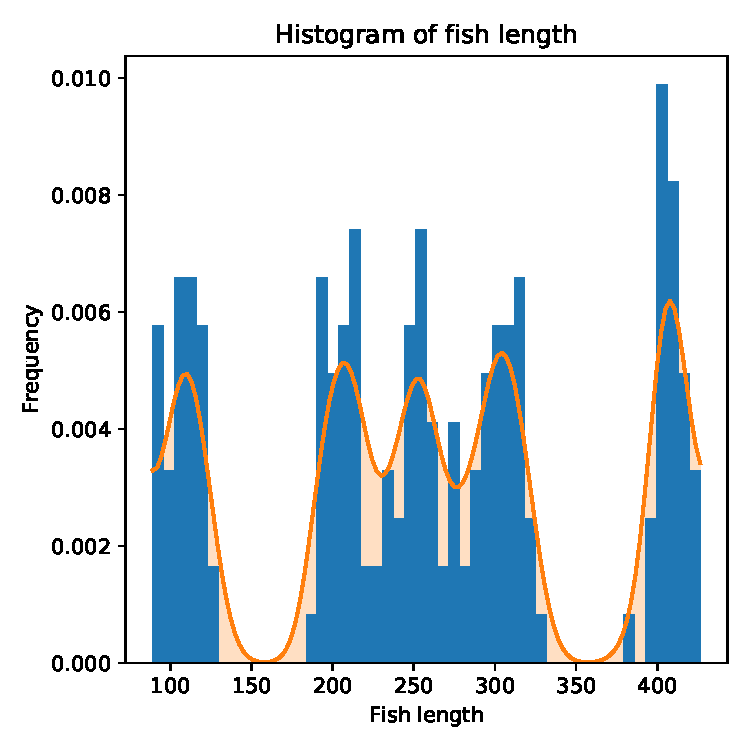
\includegraphics[scale = 0.6]{images/hist_fish_length.pdf}
    \caption{Fish length.}
    \label{Fish length}
    \end{minipage}
    \begin{minipage}[c]{0,9\textwidth}
    \centering
    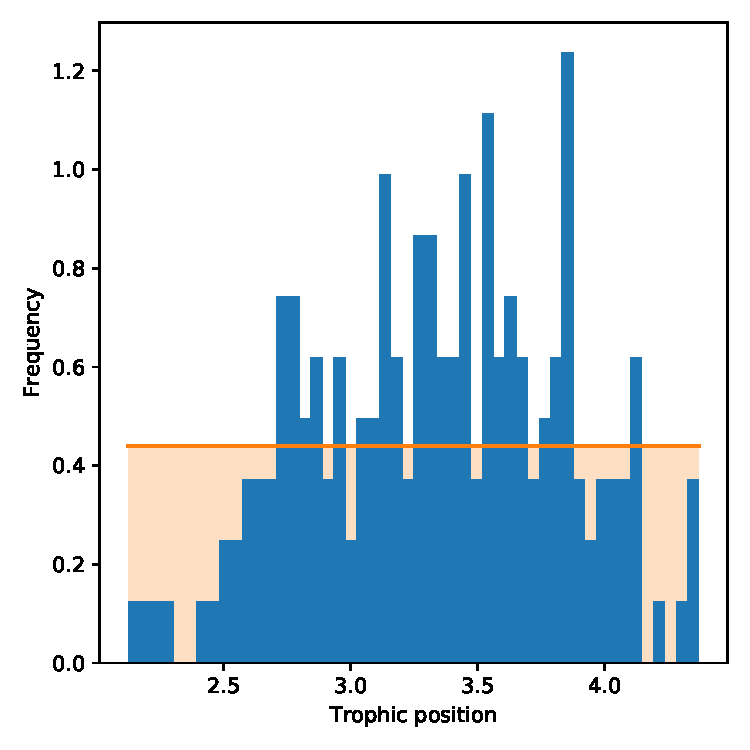
\includegraphics[scale = 0.7]{images/hist_trophic_pos.pdf}
    \caption{Trophic position.}
    \label{Trophic position}
    \end{minipage}
\end{figure}
Major deviations could cause heteroskedasticity problems, to resolve that we can apply transformations to our data.\\
We can see in Figure \ref{Fish length} and \ref{Trophic position}, that our data seems great.

We want to make sur that our scale of our data is correct. If two variables in the same model have different ranges of scale, the criteria the mixed models use to come up with parameter estimates are likely to return 'convergence errors'. Z-correction standardizes your variables and adjusts for this scaling problem by placing all your variables on the same scale even if they were originally in different units:
\begin{equation*}
    z = \left(\frac{x - \bbE[x]}{\sqrt{x}}\right)
\end{equation*}
Because the data we are dealing with have such variable scales (length is a longer scale than trophic position), we z-correct it. We do this on trophic position and fish length, and we add it to our data set. \\
To know if a mixed model is necessary for our data, we need to determine whether it is important to take into account the random effect of factors that could influence the relationship that interests us (here, Lake and Species).\\
Let us then determine whether it is important to account for variations in "random effect" by comparing
the residuals of a linear model without the random effects versus the potential random effects.
Our model is : $Z_{TP} \sim Z_{Length}$.\\
We take the stadardized residuals from the model based on the correction $Z$ done on fish length and trophic position.\\
We have the boxplot representation on Figure \ref{boxplot_lake} and \ref{boxplot_species}.\\
For this model, we should keep the random effects because the standardized residuals show variation across lake and species.
\begin{figure}[h!]
    \centering
    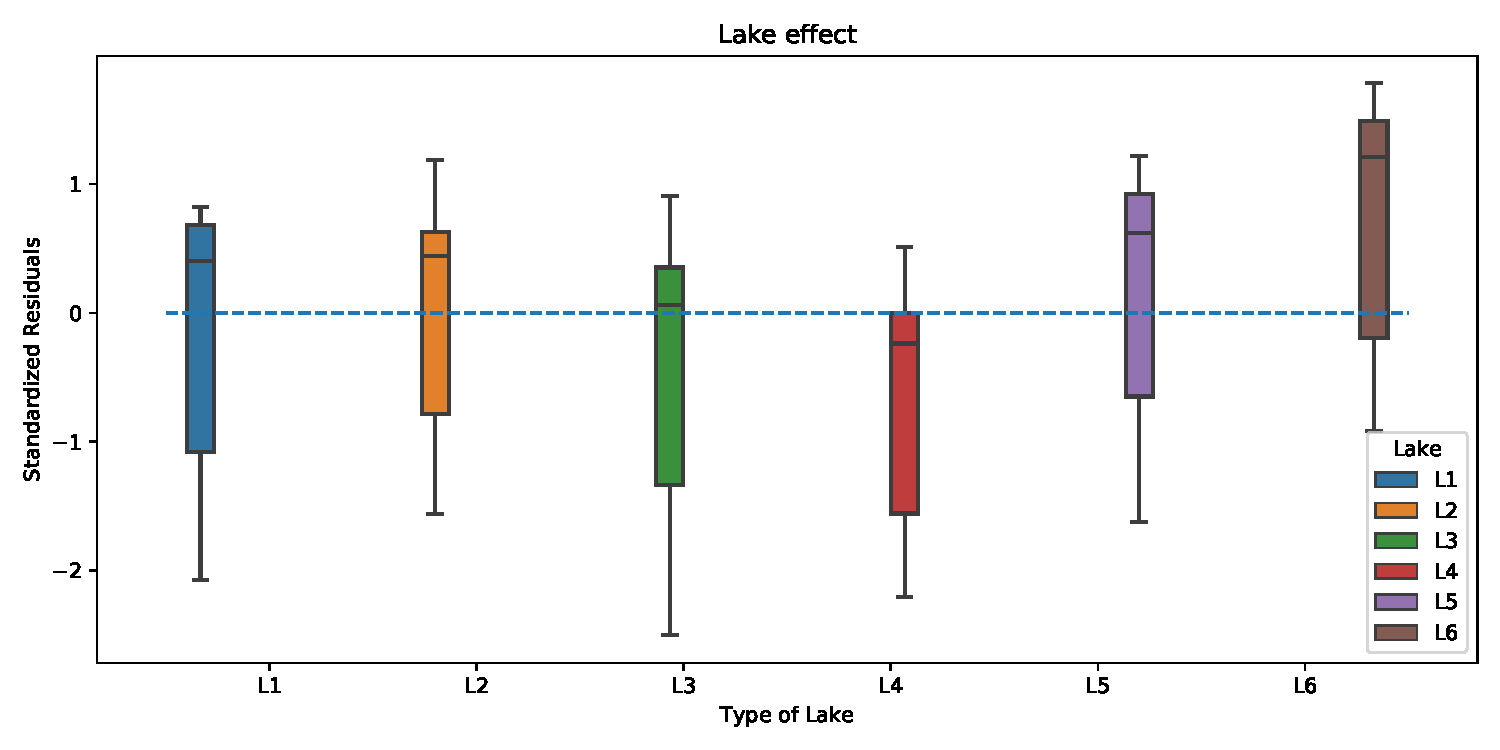
\includegraphics[scale = 0.6]{images/boxplot_lake_effect.pdf}
    \caption{Lake effect.}
    \label{boxplot_lake}
\end{figure}
    
\begin{figure}[h!]
    \centering
    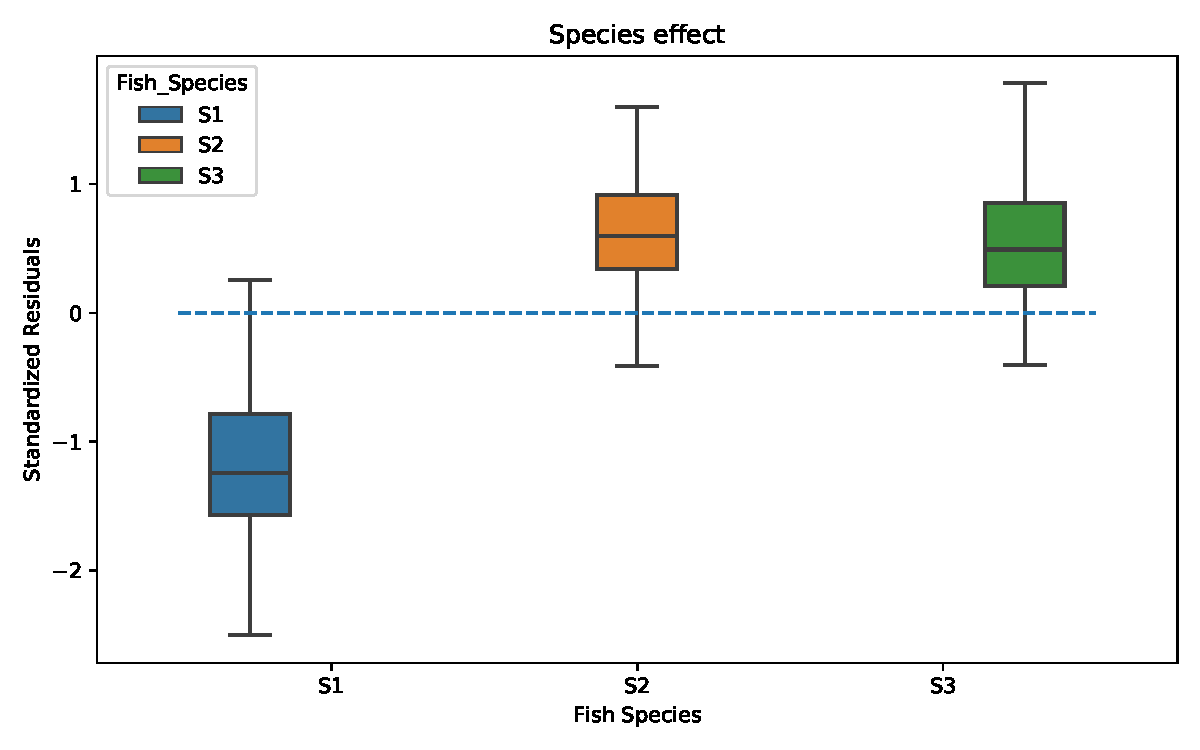
\includegraphics[scale = 0.7]{images/boxplot_species_effect.pdf}
    \caption{Fish Species effect.}
    \label{boxplot_species}
\end{figure}

\subsection{Potential models and model selection}
We have the following a priori model:
\begin{equation*}
    TP_{ijk} \sim Length_i + Lake_j + Species_k + \epsilon
\end{equation*}
We are going to do a comparison of potential models to choose the better one. We want to compare them between them to select the one (those) who has (have) the greatest predictive power, and to choose correctly we are going to use models with the lowest AIC. We will, then, compare the following models.

\begin{itemize}
    \item \textbf{Model 1:} Linear model without random effect,
    \item \textbf{Model 2:} Complete model with different intercepts, 
    \item \textbf{Model 3:} Complete model with differents intercepts and slopes,
    \item \textbf{Model 4:} No Lake effect, random intercept only,
    \item \textbf{Model 5:} No Species effect, random intercept only
    \item \textbf{Model 6:} No Lake effect, random intercept and slope,
    \item \textbf{Model 7:} No Species effect, random intercept and slope,
    \item \textbf{Model 8:} Complete model with intercepts and slopes varying by lake, 
    \item \textbf{Model 9:} Complete model with intercepts and slopes varying by species.
\end{itemize}

Then, we calculate the AIC of each model and we obtain.
\begin{table}[h!]
   \centering
    \begin{tabular}{ |p{2cm}||p{1cm}|p{1cm}|p{1cm}|p{1cm}|p{1cm}|p{1cm}|p{1cm}|p{1cm}|p{1cm}|}
    \hline
    \textbf{Models} & M1 & M2 & M3 & M4 & M5 & M6 & M7 & M8 & M9\\
    \hline
     \textbf{AIC} & 480.726 & 113.490 & 69.178 & 280.069 & 460.434 & 270.557 & 462.406 & 125.754 & 64.757\\ 
     \hline
    \end{tabular}
    \caption{AIC of each model.}
    \label{Tableau AIC}
\end{table}

We can see that, the lowest AIC is on model 9 in the Table \ref{Tableau AIC}, we choose this model as the better model.

\subsection{Model validation}

To check the assumption of homogeneity, we must plot the predicted values against the residuals. We have the graphic bellow. 
\begin{figure}[h!]
    \centering
    
\includegraphics[scale=0.7]{images/Model_validation_homo.pdf}
    \caption{Homogeneity.}
    \label{Homogeneity}
\end{figure}
The even spread of the residuals suggest that the model is a good fit for the data.

To check the assumption of homogeneity plot residuals vs each covariate in the model.\\
We have the graphics on Figure \ref{Independence}, \ref{md_val_lake} and \ref{md_val_species}.
\begin{figure}[h!]
    \begin{minipage}[c]{0,4\textwidth}
    \centering
    
\includegraphics[scale=0.6]{images/Model_validation_ind.pdf}
    \caption{Independence}
    \label{Independence}
    \end{minipage}
    \begin{minipage}[c]{0,9\textwidth}
    \centering
     
\includegraphics[scale=0.6]{images/hist_check_normality.pdf}
    \caption{Normality.}
    \label{Normality}
    \end{minipage}
\end{figure}


\begin{figure}[h!]
    \centering
    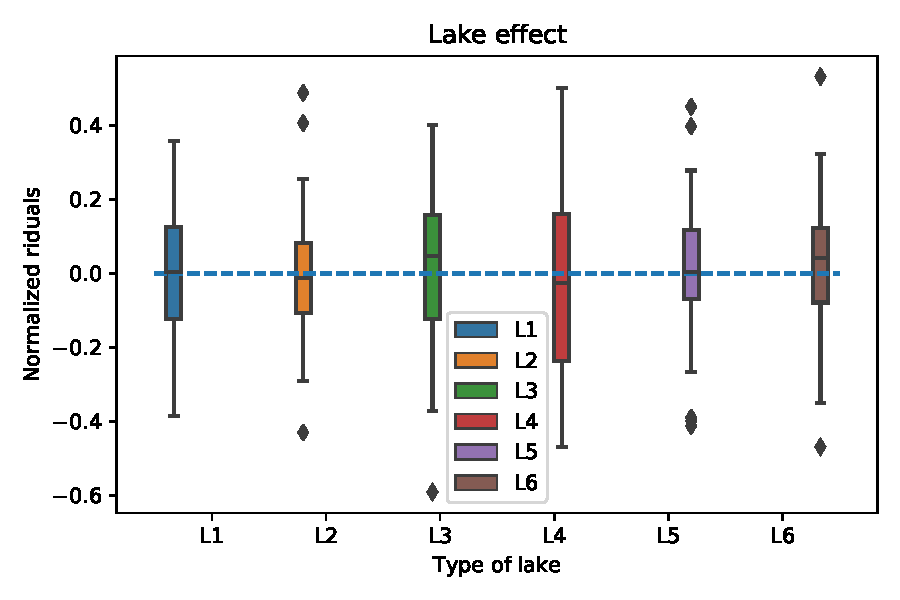
\includegraphics[scale=0.7]{images/boxplot_mod_vali_lake.pdf}
    \caption{Model validation for lake effect.}
    \label{md_val_lake}
\end{figure}
\begin{figure}[h!]
    \centering
    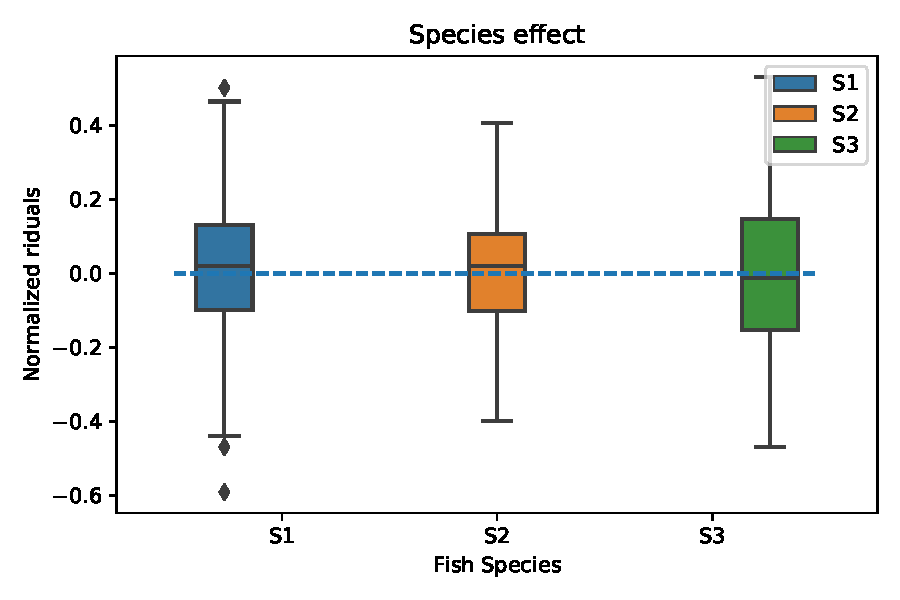
\includegraphics[scale=0.7]{images/boxplot_mod_vali_species.pdf}
    \caption{Model validation for species effect.}
    \label{md_val_species}
\end{figure}

The equal spread above and below zero indicate that there are no homogeneity problems with these variables.\\
It is also important to check the normality of the residues. Residues following a normal distribution indicate that the model is unbiased. The Figure \ref{Normality} shows that our model is unbiased.


\subsection{Interpreting results and visualizing the model}
The output is broken up into descriptions of the Random effects and Fixed effects. \\
To determine if the slope and, therefore, the effect of length on trophic position is significantly different from zero you first have to calculate the confidence interval (CI) for the slope parameter (estimate for $Z_{Length}$ in the fixed effects section = 0.4223).\\
The CI = Standard Error of the estimate $\times$ 1.96 plus or minus the parameter estimate. If the CI overlaps with zero, then the slope is not significantly different from zero at the 0.05 level. In our case, the Intercept is -0.09. So, we have, 
\begin{itemize}
    \item upper CI = 0.4223 + 0.09*1.96 = 0.5987,
    \item lower CI = 0.4223 - 0.09*1.96 = 0.2459.
\end{itemize}

As $zero$ isn't in the interval, we can say that the $Z_{Length}$ slope is significantly different from 0.\\
To visualize this model you must obtain the coefficients (intercept and slope) of each component of the model. Overall our group level model coefficients can be found in the summary of the model in the fixed effects section.
We have the following graphic. 
\begin{figure}[h!]
    \centering
    
\includegraphics[scale=0.7]{images/Model_visual_all_data.pdf}
    \caption{Model visualization of all the dataset.}
    \label{all_data}
\end{figure}

\section{Conclusion}
In our case, the trophic position increases with the size of the fish.\\

Mixed models are really good at accounting for variation in ecological data while not loosing too many degrees of freedom.\\
We have covered only a small portion of what LMM's can do. Maybe with other dataset, we will use different thing to have a great model and interpretation.

\newpage
\bibliographystyle{alpha}
\nocite{*}
\bibliography{biblio.bib}
\end{document}